\documentclass[border=10pt]{standalone}
\usepackage{pgfplots}
\pgfplotsset{compat=1.18}
\begin{document}
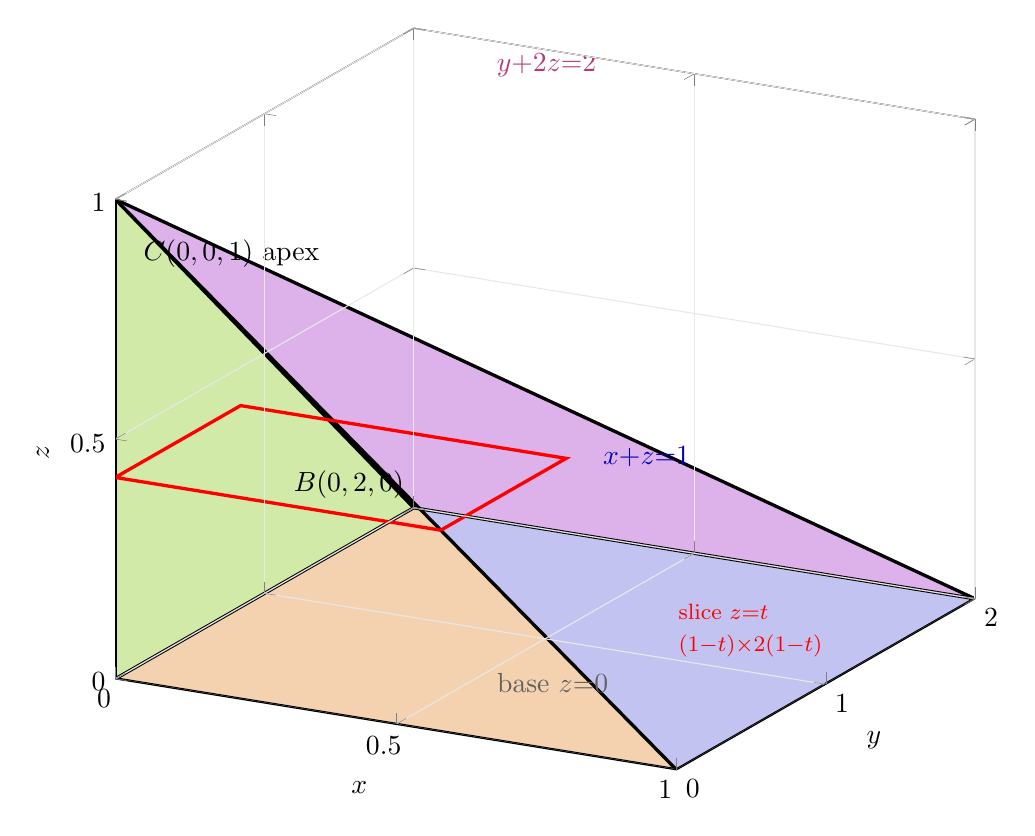
\begin{tikzpicture}
\begin{axis}[
    view={28}{22},
    width=12.5cm, height=11cm,
    xmin=0, xmax=1, ymin=0, ymax=2, zmin=0, zmax=1,
    xtick={0,0.5,1}, ytick={0,1,2}, ztick={0,0.5,1},
    xlabel=$x$, ylabel=$y$, zlabel=$z$,
    grid=major, grid style={gray!18},
    axis on top, enlargelimits=false,
    every node/.style={font=\small},
]
% ---------- faces ----------
\addplot3[fill=black!20, fill opacity=.38, draw=none] coordinates {(0,0,0) (1,0,0) (1,2,0) (0,2,0)}; % base z=0
\addplot3[fill=orange!60, fill opacity=.45, draw=none] coordinates {(0,0,0) (1,0,0) (0,0,1)};        % face y=0
\addplot3[fill=green!45,  fill opacity=.40, draw=none] coordinates {(0,0,0) (0,2,0) (0,0,1)};        % face x=0
\addplot3[fill=blue!55,   fill opacity=.33, draw=none] coordinates {(1,0,0) (1,2,0) (0,0,1)};        % x+z=1
\addplot3[fill=magenta!55,fill opacity=.33, draw=none] coordinates {(0,2,0) (1,2,0) (0,0,1)};        % y+2z=2

% ---------- edges ----------
\addplot3[very thick, draw=black] coordinates {(0,0,0) (1,0,0) (1,2,0) (0,2,0) (0,0,0)};
\addplot3[very thick, draw=black] coordinates {(1,0,0) (0,0,1) (0,2,0)};
\addplot3[very thick, draw=black] coordinates {(0,0,0) (0,0,1)};
\addplot3[very thick, draw=black] coordinates {(1,2,0) (0,0,1)};

% ---------- typical horizontal slice z = t = 0.42 ----------
\addplot3[red, very thick] coordinates {(0.58,0,0.42) (0.58,0.84,0.42) (0,0.84,0.42) (0,0,0.42) (0.58,0,0.42)};
\addplot3[red, dashed, thin] coordinates {(0,0,0) (0,0,0.42)};

% ---------- labels ----------
\node[below left]  at (axis cs:0,0,0)   {$O$};
\node[below right] at (axis cs:1,0,0)   {$A(1,0,0)$};
\node[right]       at (axis cs:1,2,0)   {$D(1,2,0)$};
\node[above left]  at (axis cs:0,2,0)   {$B(0,2,0)$};
\node[below right, black] at (axis cs:0.02,0.05,0.93) {$C(0,0,1)$ apex};
\node[blue!70!black] at (axis cs:0.92,0.10,0.62) {$x{+}z{=}1$};
\node[magenta!70!black] at (axis cs:0.25,1.95,0.98) {$y{+}2z{=}2$};
\node[black!62] at (axis cs:0.50,1.05,-0.10) {base $z{=}0$};
\node[red, align=left, font=\footnotesize] at (axis cs:1.02,0.42,0.22) {slice $z{=}t$\\[2pt] $(1{-}t){\times}2(1{-}t)$};
\end{axis}
\end{tikzpicture}
\end{document}